\documentclass{article}
\usepackage[margin=0.25in]{geometry}
\usepackage{tikz}
\usetikzlibrary{calc}

\pagenumbering{gobble}

\newcommand{\Size}{3.5cm}

\def\Sequence{1, 2, 3, 4, 5}

\tikzset{Square/.style={
    inner sep=0pt,
    text width=0.9*\Size,
    minimum size=\Size,
    line width=1pt,
    draw=black,
    align=center
    },
    font={\fontsize{13pt}{16}\selectfont}
}

\begin{document}
\begin{center}
\vspace*{\fill}{\huge\textbf{BINGO}} \\ \vspace{1.5em}

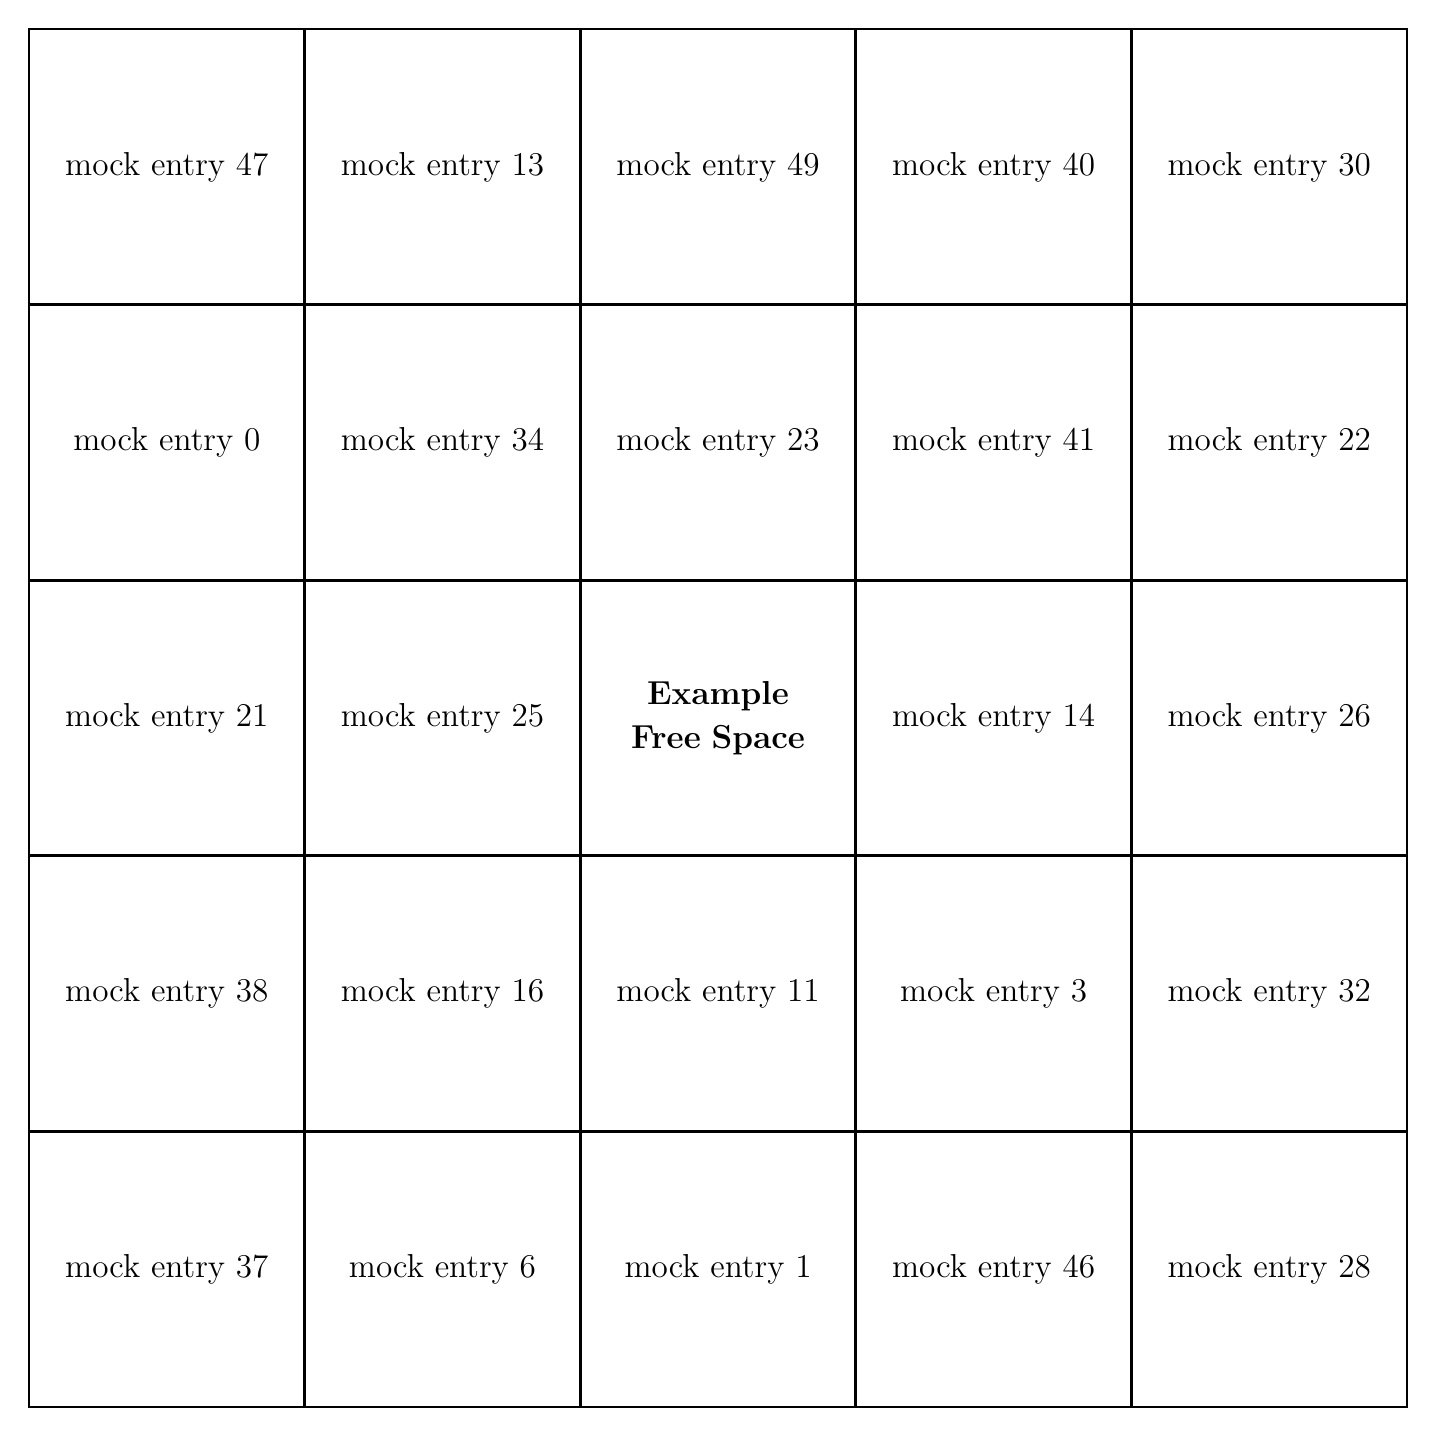
\begin{tikzpicture}[draw=black, x=\Size,y=\Size]
\foreach \col in \Sequence {
\def\row{{"mock entry 47", "mock entry 13", "mock entry 49", "mock entry 40", "mock entry 30"}}
\node [Square] at ($(\col,-1)-(0.5,0.5)$) {\pgfmathparse{\row[\col-1]}\pgfmathresult};
\def\row{{"mock entry 0", "mock entry 34", "mock entry 23", "mock entry 41", "mock entry 22"}}
\node [Square] at ($(\col,-2)-(0.5,0.5)$) {\pgfmathparse{\row[\col-1]}\pgfmathresult};
\def\row{{"mock entry 21", "mock entry 25", "\textbf{Example Free Space}", "mock entry 14", "mock entry 26"}}
\node [Square] at ($(\col,-3)-(0.5,0.5)$) {\pgfmathparse{\row[\col-1]}\pgfmathresult};
\def\row{{"mock entry 38", "mock entry 16", "mock entry 11", "mock entry 3", "mock entry 32"}}
\node [Square] at ($(\col,-4)-(0.5,0.5)$) {\pgfmathparse{\row[\col-1]}\pgfmathresult};
\def\row{{"mock entry 37", "mock entry 6", "mock entry 1", "mock entry 46", "mock entry 28"}}
\node [Square] at ($(\col,-5)-(0.5,0.5)$) {\pgfmathparse{\row[\col-1]}\pgfmathresult};
}
\end{tikzpicture}\vspace*{\fill}\newpage

\end{center}
\end{document}